\documentclass{article}

\usepackage{geometry}
\usepackage{amsmath}
\usepackage{graphicx}
\usepackage{listings}
\usepackage{hyperref}
\usepackage{multicol}
\usepackage{fancyhdr}
\pagestyle{fancy}
\hypersetup{ colorlinks=true, linkcolor=black, filecolor=magenta, urlcolor=cyan}
\geometry{ a4paper, total={170mm,257mm}, top=20mm, right=20mm, bottom=20mm, left=20mm}
\setlength{\parindent}{0pt}
\setlength{\parskip}{1em}
\renewcommand{\headrulewidth}{0pt}
\lhead{Competitive Programming - Arkavidia VI}
\fancyfoot[CE,CO]{\thepage}
\lstset{
    basicstyle=\ttfamily\small,
    columns=fixed,
    extendedchars=true,
    breaklines=true,
    tabsize=2,
    prebreak=\raisebox{0ex}[0ex][0ex]{\ensuremath{\hookleftarrow}},
    frame=none,
    showtabs=false,
    showspaces=false,
    showstringspaces=false,
    prebreak={},
    keywordstyle=\color[rgb]{0.627,0.126,0.941},
    commentstyle=\color[rgb]{0.133,0.545,0.133},
    stringstyle=\color[rgb]{01,0,0},
    captionpos=t,
    escapeinside={(\%}{\%)}
}

\begin{document}

\begin{center}
    \section*{Tantangan Penjaga Pintu} % ganti judul soal

    \begin{tabular}{ | c c | }
        \hline
        Batas Waktu  & 1s \\    % jangan lupa ganti time limit
        Batas Memori & 64MB \\  % jangan lupa ganti memory limit
        \hline
    \end{tabular}
\end{center}

\subsection*{Deskripsi}

Libur tahun baru telah tiba ! Pak Joni dan keluarga berencana berlibur di sebuah negara impiannya, Arkavland.
Arkavland memiliki $N$ buah kota yang diberi nomor dari $1$ hingga $N$. Kota - kota tersebut dihubungkan dengan $M$ buah jalan dengan aturan sebagai berikut :

\begin{enumerate}
    \setlength\itemsep{0pt}
    \item Tiap jalan yang menghubungkan kota $A$ dan $B$ memiliki panjang $1 km$
    \item Kota $A$ dan $B$ terhubung oleh maksimal sebuah rute 
    \item Jika terdapat rute dari kota $A$ ke kota $B$, rute tersebut berlaku juga sebaliknya.
\end{enumerate}

Dalam rencana liburannya yang hanya satu minggu, ia ingin berkeliling ke setiap kota, namun dia sangat pelit, sehingga Pak Joni ingin agar dapat mengeluarkan biaya seminimal mungkin dalam liburannya. 

Bantulah pak Joni mencari kota di negara Arkavland yang memiliki total jumlah jarak rute dari setiap kota lain ke kota tersebut adalah yang paling minimum.

\subsection*{Format Masukan}
Baris pertama terdiri dari dua buah bilangan $N$ dan $M$ ($1 \leq N,M \leq 10^{6}$). $N$ dan $M$ berturut-turut menyatakan banyaknya kota dan jalan di negara Arkavland.
Baris kedua hingga baris ke $M + 1$ terdiri dari dua buah bilangan $A_i$ dan $B_i$ ($1 \leq $A_i$,$B_i$ \leq N$) yang menyatakan kota $A$ dan kota $B$ terhubung oleh jalan ke-$i$

\subsection*{Format Keluaran}
Sebuah baris berisi dua bilangan $A$ dan $X$. $A$ menyatakan nomor kota yang memiliki total jumlah jarak rute dari setiap kota lain ke kota tersebut adalah yang paling minimum dan $X$ menyatakan total jumlah jaraknya. Jika terdapat banyak solusi, keluarkan jawaban dengan nomor kota yang paling kecil.
\\

\begin{multicols}{2}
\subsection*{Contoh Masukan}
\begin{lstlisting}
4 3
1 2
2 3
3 4
\end{lstlisting}
\columnbreak
\subsection*{Contoh Keluaran}
\begin{lstlisting}
2 4
\end{lstlisting}
\vfill
\null
\end{multicols}

\subsection*{Penjelasan}

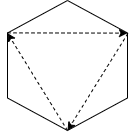
\includegraphics[width=40px]{1.png}
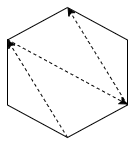
\includegraphics[width=40px]{2.png}
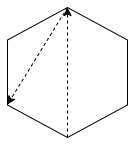
\includegraphics[width=40px]{3.png}
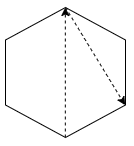
\includegraphics[width=40px]{4.png}
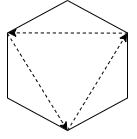
\includegraphics[width=40px]{5.png}
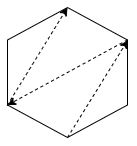
\includegraphics[width=40px]{6.png}


\pagebreak

\end{document}

